% Reconstruído de artigos/artigo_3/Artigo_3.tex


\renewcommand{\abstractname}{Resumo}
\begin{abstract}Estudamos taxas de aproximação por montagens racionais sob agendas de altura aritmética. O funcional de melhor erro define estratos, mas falha em ser homogêneo por escalares reais. Construímos aproximantes em malhas diádicas com altura suficiente de ordem $N^{\max\{1,s\}}$, com fator logarítmico para a somabilidade crítica quando $q<\infty$, e cotas uniformes sobre bolas de Besov. Para erro bruto de ordem $N^{-\alpha}$ e crescimento de Lipschitz $N^\gamma$, obtemos regularidade inversa de ordem $\alpha/(\alpha+\gamma)$; um pente de tendas demonstra agudeza na biblioteca original quando $0<\alpha\le\gamma$. A extensão marcada caracteriza a reversibilidade exata com redes ReLU rasas racionais, e uma construção quantizada trata parâmetros reais. Ao somar ao erro a segunda diferença do aproximante na escala correspondente, obtemos uma caracterização direta e inversa das classes de Besov. A cota inversa desse funcional é universal; a direção direta fornece o controle aritmético específico da biblioteca.\end{abstract}
\renewcommand{\abstractname}{Abstract}
\begin{abstract}We study approximation rates of rational assemblies under arithmetic height schedules. The best-error functional defines approximation strata but fails real homogeneity. We construct dyadic approximants with sufficient height of order $N^{\max\{1,s\}}$, with a logarithmic factor for critical summability when $q<\infty$, and uniform bounds on Besov balls. A raw rate $N^{-\alpha}$ under Lipschitz growth $N^\gamma$ implies inverse regularity of order $\alpha/(\alpha+\gamma)$; a tent comb proves sharpness in the original library for $0<\alpha\le\gamma$. A marked completion characterizes exact reversal of rational shallow ReLU networks, while quantization handles real parameters. Adding the approximant's second-order modulus at the matching scale yields a direct and inverse characterization of Besov classes. The inverse bound is universal; the direct construction supplies the arithmetic control specific to the library.\end{abstract}
\renewcommand{\abstractname}{Resumo}
\section{Introdução}
Uma função linear por partes pode ter erro de aproximação nulo em todas as escalas posteriores e conservar quinas. Por isso, uma taxa rápida do melhor erro, tomada isoladamente, não caracteriza suavidade de ordem superior a um. Sob restrições aritméticas, soma-se outra questão: o catálogo de altura fixa não é invariante por multiplicação por escalares reais.

Este artigo formula as classes de aproximação compatíveis com essa estrutura e estabelece suas relações com espaços de Besov. A biblioteca e os resultados de custo e seleção foram desenvolvidos nos dois primeiros artigos \citep{artigo_2-oliveiraI,artigo_2-oliveiraII}. A teoria de aproximação não linear e os teoremas diretos e inversos fornecem o contexto funcional \citep{artigo_1-devore1998,artigo_2-devorepopov1988,artigo_2-petrushev1988,artigo_2-devorelorentz1993}. Funcionais de realização relacionam aproximação restrita e módulos de suavidade \citep{artigo_2-hristovivanov1990}. As relações com redes ReLU e restrições de pesos são tratadas em \citet{artigo_2-devorehaninpetrova2021,artigo_1-daubechies2022,artigo_2-gribonval2022,artigo_2-grohs2023,artigo_1-guhring2021}.

O primeiro resultado acompanha o denominador racional comum e fornece agendas suficientes de altura. O segundo relaciona erro bruto e crescimento das inclinações a uma regularidade inversa com perda. A agudeza na biblioteca original é demonstrada na faixa $0<\alpha\le\gamma$. A reversibilidade exata com redes rasas exige parâmetros racionais e quebras diádicas; a extensão marcada conserva explicitamente o suporte de peças constantes.

Para recuperar uma caracterização de Besov, somamos ao erro o módulo de segunda ordem do aproximante na escala pareada. A desigualdade inversa vale para qualquer família de funções. A racionalização estabelece a direção direta com altura controlada, inclusive uniformemente sobre bolas. As igualdades obtidas são igualdades de conjuntos sob as agendas declaradas.

\section{Biblioteca, altura e erro de aproximação}
\label{artigo_3:sec:baseIII}
Usamos a biblioteca racional do primeiro artigo \citep{artigo_2-oliveiraI} e o controle de recursos do segundo \citep{artigo_2-oliveiraII}. Para $r=p/q$ reduzido, $q>0$, ponha $\height(r)=\max\{|p|,q\}$. Um átomo em $J_{k,m}=[m2^{-k},(m+1)2^{-k}]$ tem a forma
\begin{equation}
 \ell(x)=y_0+s(x-x_{k,m}),\quad x_{k,m}=(m+1/2)2^{-k},\quad y_0\in\mathbb Q,\ s\in\Qstar,
 \label{artigo_3:eq:inherited-atom}
\end{equation}
e altura
\begin{equation}
 \height_{\rm at}=\max\{2,k+1,|m|+1,\height(y_0),\height(s)\}.
 \label{artigo_3:eq:inherited-height}
\end{equation}
Fixe uma raiz $K=J_{k_0,m_0}$. Uma montagem é uma função contínua que coincide com um átomo em cada folha de uma árvore diádica finita com raiz $K$. Escreva $\Aclass_{N,H}(K)$ para as funções que admitem uma mesma representação com até $N$ folhas e altura máxima $H$, e
\[
 E_{N,H}^{\Library}(f)_\infty=\inf_{g\in\Aclass_{N,H}(K)}\|f-g\|_{\infty,K}.
\]
Os catálogos são finitos, pois a altura limita todas as coordenadas atômicas. Ao longo de orçamentos cofinalmente crescentes, suas montagens são densas em $C(K)$.

Na malha uniforme de $n=2^r$ folhas, os índices são $(k_0+r,2^rm_0+j)$, $0\le j<n$. Se $m_0\ge0$, a admissibilidade geométrica de todas as folhas equivale a $k_0+r+1\le H$ e $n(m_0+1)\le H$. Em particular, em $[0,1]$ a malha uniforme exige $H\ge n$.

O segundo artigo demonstra que, para $\mathcal F_{R,M}=\{f\in C^2[0,1]:\|f\|_\infty\le R,\ \|f''\|_\infty\le M\}$ e $C_H=\max\{4(R+1),2(4R+M/2+1)\}$,
\[
 E_{N,\lceil C_HN^2\rceil}^{\Library}(f)_\infty<\frac{M+4}{2N^2},\qquad N\ge2.
\]
A construção usa valores nodais racionais em grades alternadas, preserva inclinações não nulas e admite $O_{R,M}(N\log(2N))$ bits nos formatos atômico, ReLU estrutural e ReLU racional. Esses resultados fornecem o endpoint $C^2$ usado adiante.

\section{Classes de aproximação sob uma agenda de altura}
\label{artigo_3:sec:approximation-classes}

O número de folhas e a altura aritmética desempenham papéis independentes. A
racionalização por denominador comum absorve o fator da malha e fornece
altura suficiente $N^2$ no caso $s=2$. Ao mesmo tempo, catálogos racionais de
altura fixa falham em ser invariantes por escalares reais. O funcional
associado será, por isso, formulado como funcional de taxa e sua obstrução de
homogeneidade será demonstrada explicitamente.

\subsection{Erro apontado e funcional de taxa}

Seja $H:\mathbb N\to\mathbb N$, $H(N)\ge2$, uma agenda não decrescente.
Estenda a notação $\Aclass_{N,H}(K)$ ao caso $N=1$ pela mesma
definição: no máximo uma folha e altura no máximo $H$. Essa classe pode não
conter a função nula, pois a
biblioteca exclui inclinações nulas. Para obter um erro com ponto-base sem
alterar nenhum aproximante não nulo, ponha
\begin{equation}
 \Sigma_N^{\Library,H}(K)
 :=\{0\}\cup\Aclass_{N,H(N)}(K),
 \qquad
 e_N^{\Library,H}(f)
 :=\inf_{g\in\Sigma_N^{\Library,H}(K)}\|f-g\|_{\infty,K}.
 \label{artigo_3:eq:pointed-error}
\end{equation}
Em termos do erro conjunto da seção de custos do segundo artigo \citep{artigo_2-oliveiraII}, estendido pela mesma fórmula
ao caso $N=1$,
\begin{equation}
 e_N^{\Library,H}(f)
 =\min\bigl\{\|f\|_{\infty,K},
 E_{N,H(N)}^{\Library}(f)_\infty\bigr\}.
 \label{artigo_3:eq:pointed-inherited}
\end{equation}
A origem completa o esquema apontado usado para medir taxas.

% MAPA artigo_3:3.1
\begin{proposition}[aninhamento da agenda]\label{map:artigo_3:3.1}
\label{artigo_3:prop:schedule-nesting}
Se $H$ é não decrescente, então
\begin{equation}
 \Sigma_N^{\Library,H}(K)
 \subseteq\Sigma_{N+1}^{\Library,H}(K)
 \quad\text{e}\quad
 e_{N+1}^{\Library,H}(f)\le e_N^{\Library,H}(f)\le\|f\|_\infty.
 \label{artigo_3:eq:schedule-nesting}
\end{equation}
Para cada $N$, o ínfimo em \eqref{artigo_3:eq:pointed-error} é atingido.
\end{proposition}

\begin{proof}
Uma representação com no máximo $N$ folhas e altura no máximo $H(N)$
continua admissível sob os limites $N+1$ e $H(N+1)$. A função nula pertence
a ambas as classes. Isso prova as inclusões e as desigualdades. O calibre de
altura limita escala, translação, valor central e inclinação; portanto há
somente um número finito de átomos e de árvores admissíveis. Assim
$\Sigma_N^{\Library,H}(K)$ é finito e a distância mínima é atingida.
\end{proof}

A definição de classes por sequências de melhores erros é padrão na teoria de
espaços de aproximação não linear \citep{artigo_1-devore1998}. O funcional seguinte
acrescenta a essa construção o catálogo apontado e a agenda aritmética de
altura.

Para $\alpha>0$ e $0<q\le\infty$, defina o \emph{funcional de taxa}
\begin{align}
 \mathfrak a_{\alpha,q}^{\Library,H}(f)
 &:=\left(\sum_{N=1}^{\infty}
       \bigl[N^\alpha e_N^{\Library,H}(f)\bigr]^q\frac1N
       \right)^{1/q}, &&0<q<\infty,
 \label{artigo_3:eq:rate-functional-finite}\\
 \mathfrak a_{\alpha,\infty}^{\Library,H}(f)
 &:=\sup_{N\ge1}N^\alpha e_N^{\Library,H}(f).
 \label{artigo_3:eq:rate-functional-infty}
\end{align}
Escreva
\begin{equation}
 \mathscr A_{q}^{\alpha}(\Library,H)
 :=\{f\in C(K):\mathfrak a_{\alpha,q}^{\Library,H}(f)<\infty\}.
 \label{artigo_3:eq:approximation-stratum}
\end{equation}
O termo \emph{classe} ou \emph{estrato} será usado para
\eqref{artigo_3:eq:approximation-stratum}; \emph{espaço quase-normado} será reservado
a situações em que homogeneidade e quase-triângulo tenham sido efetivamente
provados. Essa distinção é necessária no catálogo presente e não ocorre
automaticamente a partir da literatura de esquemas cônicos ou de redes
\citep{artigo_2-gribonval2022,artigo_2-grohs2023}.

% MAPA artigo_3:3.2
\begin{theorem}[redução exata às escalas diádicas]\label{map:artigo_3:3.2}
\label{artigo_3:thm:dyadic-rate-equivalence}
Para toda agenda não decrescente, $\alpha>0$ e $0<q\le\infty$,
\begin{equation}
 \mathfrak a_{\alpha,q}^{\Library,H}(f)
 \asymp_{\alpha,q}
 \left\|\bigl(2^{r\alpha}
 e_{2^r}^{\Library,H}(f)\bigr)_{r\ge0}\right\|_{\ell^q},
 \label{artigo_3:eq:dyadic-rate-equivalence}
\end{equation}
com a interpretação usual por supremo quando $q=\infty$. As constantes não
dependem de $f$ nem de $H$.
\end{theorem}

\begin{proof}
No bloco $2^r\le N<2^{r+1}$, a monotonicidade fornece
\[
 e_{2^{r+1}}^{\Library,H}(f)
 \le e_N^{\Library,H}(f)
 \le e_{2^r}^{\Library,H}(f),
\]
enquanto $2^{r\alpha}\le N^\alpha<2^{(r+1)\alpha}$ e
\[
 \sum_{N=2^r}^{2^{r+1}-1}\frac1N\asymp1.
\]
Somar as duas estimativas de bloco e deslocar o índice inferior por uma
unidade prova \eqref{artigo_3:eq:dyadic-rate-equivalence}. Para $q=\infty$, basta
tomar o supremo nos mesmos blocos.
\end{proof}

\subsection{Obstrução de homogeneidade}

% MAPA artigo_3:3.3
\begin{proposition}[falha exata de homogeneidade]\label{map:artigo_3:3.3}
\label{artigo_3:prop:nonhomogeneous-functional}
Suponha $K=[0,1]$ e $H(1)\ge2$. O funcional
$\|f\|_\infty+\mathfrak a_{\alpha,q}^{\Library,H}(f)$ não é homogêneo sobre
$C(K)$ e, portanto, não é uma quase-norma. Mais precisamente, para
$f(x)=x$ e $c=\sqrt2$,
\begin{equation}
 \mathfrak a_{\alpha,q}^{\Library,H}(f)=0,
 \qquad
 \mathfrak a_{\alpha,q}^{\Library,H}(cf)>0.
 \label{artigo_3:eq:nonhomogeneous-certificate}
\end{equation}
\end{proposition}

\begin{proof}
A função $f(x)=x$ é o átomo $(k,m,y_0,s)=(0,0,1/2,1)$, de altura $2$.
Logo $f\in\Sigma_N^{\Library,H}(K)$ para todo $N$ e todos os erros de
$f$ são nulos. Por outro lado, toda função não nula em
$\Sigma_1^{\Library,H}(K)$ possui inclinação racional em $[0,1]$, enquanto
$cf$ possui inclinação irracional $\sqrt2$. Como o primeiro catálogo é
finito, $cf$ tem distância estritamente positiva a ele. Assim o termo
$N=1$ de \eqref{artigo_3:eq:rate-functional-finite}, ou o mesmo termo no supremo,
é positivo. Consequentemente,
\[
 \|cf\|_\infty+\mathfrak a_{\alpha,q}^{\Library,H}(cf)
 >|c|\bigl(\|f\|_\infty+
 \mathfrak a_{\alpha,q}^{\Library,H}(f)\bigr).
\]
\end{proof}

% MAPA artigo_3:3.4
\begin{remark}[estrutura aritmética do funcional]\label{map:artigo_3:3.4}
\label{artigo_3:rem:quasinorm-scope}
Adicionar $0$ fornece o ponto-base, enquanto a obstrução de homogeneidade real
permanece. O fecho cônico ou o envoltório linear admite escalares reais
externos e elimina o custo aritmético medido por $H$. Assim, os objetos
naturais são os estratos \eqref{artigo_3:eq:approximation-stratum} e seus funcionais de
taxa.
\end{remark}

\section{Teoremas diretos e agendas de altura}
\label{artigo_3:sec:direct-height}

O paradigma de teoremas diretos e inversos tem antecedentes tanto na
aproximação por splines e em espaços de Besov quanto na aproximação por funções
racionais \citep{artigo_2-petrushev1988,artigo_2-petrushevpopov1987}. Nesta última expressão,
``racional'' significa quociente de polinômios, e não a aritmética dos
coeficientes da biblioteca; o elemento novo desta seção é acompanhar
explicitamente a altura desses coeficientes.

Fixe a raiz diádica $K=J_{k_0,m_0}$ e escreva $L=|K|=2^{-k_0}$. Para
$f\in C(K)$, defina
\begin{align}
 \omega_1(f,t)_{\infty,K}
 &=\sup_{\substack{0<h\le t\\x,x+h\in K}}
   |f(x+h)-f(x)|,\label{artigo_3:eq:first-modulus}\\
 \omega_2(f,t)_{\infty,K}
 &=\sup_{\substack{0<h\le t\\x,x+2h\in K}}
   |f(x+2h)-2f(x+h)+f(x)|.
 \label{artigo_3:eq:second-modulus-direct}
\end{align}
Para $0<s<2$ e $0<q\le\infty$, usaremos a caracterização diádica equivalente da
quase-norma de Besov
\begin{equation}
 \|f\|_{B^s_{\infty,q}(K)}^*
 :=\|f\|_{\infty,K}
 +\left\|\bigl(2^{rs}\omega_2(f,L2^{-r})_{\infty,K}
           \bigr)_{r\ge0}\right\|_{\ell^q}.
 \label{artigo_3:eq:dyadic-besov-norm}
\end{equation}
Ela é equivalente à definição integral com medida $\dd t/t$; essa
discretização é clássica e decorre das desigualdades de escala do módulo de
suavidade \citep{artigo_2-devorelorentz1993,artigo_2-devorepopov1988}.

Também será usada a desigualdade de Whitney de ordem dois
\citep{artigo_2-whitney1957,artigo_1-devore1998}: existe uma
constante universal $C_W$ tal que, em todo subintervalo $J\subset K$,
\begin{equation}
 \inf_{\ell\ \text{afim}}\|f-\ell\|_{\infty,J}
 \le C_W\omega_2(f,|J|)_{\infty,J}.
 \label{artigo_3:eq:whitney-direct}
\end{equation}
Como o interpolador nos extremos reproduz funções afins e tem norma de
operador $1$, seu erro é no máximo duas vezes o lado direito.

Ponha
\begin{equation}
 \nu_s=\max\{1,s\},
 \qquad C_K=4(k_0+|m_0|+2).
 \label{artigo_3:eq:height-schedule-constants}
\end{equation}

\subsection{Racionalização com denominador comensurável}

A prova precisa acompanhar também primeiras diferenças. A desigualdade de
Marchaud de ordens um e dois
\citep{artigo_2-devorelorentz1993,artigo_1-lorentz1996} implica, para $0<t\le L/2$,
\begin{equation}
 \omega_1(f,t)_{\infty,K}
 \le C_s\|f\|_{B^s_{\infty,\infty}(K)}^*
 \begin{cases}
  (t/L)^s,&0<s<1,\\
  (t/L)\log(eL/t),&s=1,\\
  t/L,&1<s<2.
 \end{cases}
 \label{artigo_3:eq:marchaud-regimes}
\end{equation}
Essa estimativa limita a inclinação quando
o denominador disponível é menor que o inverso da malha.

% MAPA artigo_3:4.1
\begin{lemma}[Jackson racional com altura explícita]\label{map:artigo_3:4.1}
\label{artigo_3:lem:rational-jackson-height}
Seja $f\in B^s_{\infty,\infty}(K)$, $R=\|f\|_\infty$. Existe
$n_0=n_0(f,K,s)$ tal que, para toda potência de dois $n=2^r\ge n_0$ e todo
inteiro
\[
 H\ge\max\{C_Kn^{\nu_s},16(R+1)\}
\]
que satisfaça
\begin{equation}
 H\ge\max\{2,k_0+r+1,
      \max_{0\le j<n}|2^rm_0+j|+1\},
 \label{artigo_3:eq:height-geometry-condition}
\end{equation}
existe $g_{n,H}\in\Aclass_{n,H}(K)$ tal que
\begin{equation}
 \|f-g_{n,H}\|_\infty
 \le 2C_W\omega_2(f,L/n)_{\infty,K}
      +\frac{C(R+1)}{H},
 \label{artigo_3:eq:rational-jackson-height}
\end{equation}
onde $C$ é absoluto e $C_W$ é a constante de Whitney.

Além disso, existe $A_{K,s}\ge1$, independente de $f$, com a seguinte versão
uniforme. Se $B\ge1$, $\|f\|_{B^s_{\infty,\infty}(K)}^*\le B$, $n=2^r\ge2$
e
\begin{equation}
 H\ge A_{K,s}(B+1)n^{\nu_s},
 \label{artigo_3:eq:uniform-ball-height-threshold}
\end{equation}
então todas as conclusões anteriores valem sem limiar dependente de $f$ e com
o último termo de \eqref{artigo_3:eq:rational-jackson-height} igual a
$8(B+1)/H$. A constante $A_{K,s}$ também torna automática a condição
geométrica \eqref{artigo_3:eq:height-geometry-condition}.
\end{lemma}

\begin{proof}
Escolha a maior potência de dois $Q$ tal que
$8(R+1)Q\le H$. Para $H\ge16(R+1)$,
\begin{equation}
 \frac{H}{16(R+1)}<Q\le\frac{H}{8(R+1)}.
 \label{artigo_3:eq:Q-window}
\end{equation}
Nos nós $t_j=\inf K+jL/n$, use as grades alternadas
\[
 G_j=\frac1Q\left(\mathbb Z+\frac{j\bmod2}{2}\right)
\]
e escolha $v_j\in G_j$ mais próximo de $f(t_j)$; se os dois vizinhos da grade
forem equidistantes, escolha o menor. Então
$|v_j-f(t_j)|\le(2Q)^{-1}$ e $v_j\ne v_{j+1}$. Escrevendo
$v_j=b_j/(2Q)$ com $b_j\equiv j\pmod2$, obtém-se
\begin{equation}
 |b_j|\le2QR+1.
 \label{artigo_3:eq:general-b-bound}
\end{equation}
Na célula $J_{k_0+r,2^rm_0+j}$, os parâmetros são
\begin{equation}
 y_{0,j}=\frac{b_j+b_{j+1}}{4Q},
 \qquad
 s_j=2^{k_0+r}\frac{b_{j+1}-b_j}{2Q}.
 \label{artigo_3:eq:general-atom-parameters}
\end{equation}
A janela \eqref{artigo_3:eq:Q-window} e \eqref{artigo_3:eq:general-b-bound} dão
$\height(y_{0,j})\le H$. Como $b_{j+1}-b_j$ é ímpar, não há cancelamento
oculto com $2Q$. Se $2^{k_0+r}\le2Q$, a fração reduzida de $s_j$ tem
numerador $b_{j+1}-b_j$ e denominador $2Q/2^{k_0+r}$; a cota grosseira
$|b_{j+1}-b_j|\le4QR+2$ prova $\height(s_j)\le H$ após um aumento absoluto
do limiar inicial.

Se $2^{k_0+r}>2Q$, a inclinação é inteira e
\begin{equation}
 |s_j|
 \le \frac nL\left(\omega_1(f,L/n)+\frac1Q\right).
 \label{artigo_3:eq:slope-marchaud-bound}
\end{equation}
Nos três regimes de \eqref{artigo_3:eq:marchaud-regimes}, o primeiro termo é limitado,
respectivamente, por
\[
 C_{K,s}\|f\|_{B^s_{\infty,\infty}}^*n^{1-s},\qquad
 C_{K}\|f\|_{B^1_{\infty,\infty}}^*\log(en),\qquad
 C_{K,s}\|f\|_{B^s_{\infty,\infty}}^*;
\]
o segundo é $O((R+1)n/H)$. Com o coeficiente fixo da primeira parte, essas
quantidades ficam abaixo de $H$ quando $n\ge n_0(f,K,s)$. Se a norma é no
máximo $B$, as desigualdades elementares
$n^{1-s}\le n$, $\log(en)\le2n$ e $1\le n^{\nu_s}$, juntamente com
\eqref{artigo_3:eq:uniform-ball-height-threshold}, dão a mesma conclusão para todo
$n\ge2$ após escolher $A_{K,s}$ suficientemente grande. Como
\[
 k_0+r+1\le C_Kn,\qquad
 \max_{0\le j<n}|2^rm_0+j|+1\le(|m_0|+1)n+1,
\]
essa escolha também cobre a geometria. Logo cada peça pertence a
$\Library_H$ em ambas as versões.

Se $P_nf$ é o interpolante dos valores exatos nos mesmos nós, a estimativa
de Whitney \eqref{artigo_3:eq:whitney-direct} dá
\[
 \|f-P_nf\|_\infty
 \le2C_W\omega_2(f,L/n)_{\infty,K}.
\]
A diferença entre os dois interpolantes é, em cada célula, uma combinação
convexa dos erros nodais e não excede $(2Q)^{-1}$. Usando
\eqref{artigo_3:eq:Q-window}, esse termo é estritamente menor que
$8(R+1)/H\le8(B+1)/H$ na versão uniforme. Isso prova as duas afirmações.
\end{proof}

\subsection{Imersões diretas com altura controlada}

Para $\kappa\ge0$, defina a agenda inteira
\begin{equation}
 H_{s,\kappa}(N)
 =\left\lceil C_K(N+1)^{\nu_s}
        [\log(eN)]^\kappa\right\rceil.
 \label{artigo_3:eq:corrected-height-schedule}
\end{equation}
Ela é não decrescente e satisfaz a obstrução geométrica de
\eqref{artigo_3:eq:height-geometry-condition} em toda malha uniforme com no máximo
$N$ folhas.

% MAPA artigo_3:4.2
\begin{theorem}[direção direta com altura aritmética]\label{map:artigo_3:4.2}
\label{artigo_3:thm:direct-besov-height}
Se $0<s<2$, então as seguintes inclusões de conjuntos valem:
\begin{align}
 B^s_{\infty,\infty}(K)
 &\subset
 \mathscr A^s_\infty(\Library,H_{s,0}),
 \label{artigo_3:eq:direct-endpoint}\\
 B^s_{\infty,q}(K)
 &\subset
 \mathscr A^s_q(\Library,H_{s,0}),
 &&0<q<\infty,\qquad 0<s<1,
 \label{artigo_3:eq:direct-subcritical}\\
 B^s_{\infty,q}(K)
 &\subset
 \mathscr A^s_q(\Library,H_{s,\kappa}),
 &&0<q<\infty,\qquad 1\le s<2,\qquad\kappa>1/q.
 \label{artigo_3:eq:direct-critical-log}
\end{align}
Em particular, para $s\ge1$, o endpoint $q=\infty$ admite
$H(N)=O_K(N^s)$; para $q<\infty$, basta acrescentar um fator logarítmico
crítico. Como
alternativa sem logaritmo, para qualquer $\eta>0$ pode-se substituir
$H_{s,\kappa}$ em \eqref{artigo_3:eq:direct-critical-log} por
\begin{equation}
 \widetilde H_{s,\eta}(N)
 =\left\lceil C_K(N+1)^{\max\{1,s+\eta\}}\right\rceil.
 \label{artigo_3:eq:polynomial-slack-schedule}
\end{equation}
\end{theorem}

\begin{proof}
Seja $n=2^r$. Para $r$ suficientemente grande, o
\cref{artigo_3:lem:rational-jackson-height} aplicado a
$H=H_{s,\kappa}(n)$ dá
\begin{equation}
 n^s e_n^{\Library,H}(f)
 \le C n^s\omega_2(f,L/n)_{\infty,K}
     +C_f\frac{n^s}{H_{s,\kappa}(n)}.
 \label{artigo_3:eq:direct-sequence-bound}
\end{equation}
Um número finito de escalas iniciais não afeta pertinência a $\ell^q$. O
primeiro termo do lado direito pertence a $\ell^q$ por
\eqref{artigo_3:eq:dyadic-besov-norm}. Se $s<1$, o segundo decai geometricamente como
$n^{s-1}$. Se $s\ge1$, ele é $O(r^{-\kappa})$, pois
$\log(en)\asymp r$; pertence a $\ell^q$ quando $\kappa q>1$ e é limitado
quando $q=\infty$ e $\kappa=0$. A agenda
\eqref{artigo_3:eq:polynomial-slack-schedule} produz, em vez disso, o fator
$n^{-\eta}$. O \cref{artigo_3:thm:dyadic-rate-equivalence} transfere as conclusões
das potências de dois para todos os orçamentos $N$.
\end{proof}

A versão uniforme do \cref{artigo_3:lem:rational-jackson-height} calibra uma agenda para cada bola de Besov. As cotas são formuladas sobre bolas porque o funcional de taxa satisfaz a obstrução de homogeneidade da \cref{artigo_3:prop:nonhomogeneous-functional}.

% MAPA artigo_3:4.3
\begin{corollary}[imersões quantitativas uniformes sobre bolas]\label{map:artigo_3:4.3}
\label{artigo_3:cor:uniform-besov-ball-embedding}
Para $B\ge1$ e $\kappa\ge0$, defina
\begin{equation}
 \widehat H_{s,\kappa}^{[B]}(N)
 =\left\lceil A_{K,s}(B+1)(N+1)^{\nu_s}
        [\log(eN)]^\kappa\right\rceil .
 \label{artigo_3:eq:ball-calibrated-height-schedule}
\end{equation}
Existem constantes independentes de $B$ e de $f$ tais que
\begin{align}
 \sup_{\|f\|_{B^s_{\infty,\infty}(K)}^*\le B}
 \mathfrak a_{s,\infty}^{\Library,
       \widehat H_{s,0}^{[B]}}(f)
 &\le C_{K,s}(B+1), &&0<s<2,\label{artigo_3:eq:uniform-ball-endpoint}\\
 \sup_{\|f\|_{B^s_{\infty,q}(K)}^*\le B}
 \mathfrak a_{s,q}^{\Library,
       \widehat H_{s,0}^{[B]}}(f)
 &\le C_{K,s,q}(B+1), &&0<s<1,\quad0<q<\infty,
 \label{artigo_3:eq:uniform-ball-subcritical}\\
 \sup_{\|f\|_{B^s_{\infty,q}(K)}^*\le B}
 \mathfrak a_{s,q}^{\Library,
       \widehat H_{s,\kappa}^{[B]}}(f)
 &\le C_{K,s,q,\kappa}(B+1),
 &&1\le s<2,\quad0<q<\infty,\quad\kappa>1/q.
 \label{artigo_3:eq:uniform-ball-critical}
\end{align}
Assim, cada bola de Besov é enviada uniformemente a uma bola do funcional de
taxa sob uma única agenda, sem qualquer limiar dependente da função.
\end{corollary}

\begin{proof}
Para $n=2^r\ge2$, a versão uniforme do
\cref{artigo_3:lem:rational-jackson-height} fornece
\[
 n^s e_n^{\Library,\widehat H}(f)
 \le C_{K,s}n^s\omega_2(f,L/n)_{\infty,K}
 +C_{K,s}\frac{n^s}{n^{\nu_s}[\log(en)]^\kappa}.
\]
O primeiro termo tem norma $\ell^q$ limitada por $C_{K,s}B$ na
caracterização \eqref{artigo_3:eq:dyadic-besov-norm}. O segundo é limitado para
$q=\infty$; é geometricamente somável se $s<1$ e $\kappa=0$; e pertence a
$\ell^q$ se $s\ge1$ e $\kappa q>1$. A escala $N=1$ é limitada por
$\|f\|_\infty\le B$. A equivalência diádica do
\cref{artigo_3:thm:dyadic-rate-equivalence} conclui as três cotas.
\end{proof}

% MAPA artigo_3:4.4
\begin{remark}[o papel do índice $q$]\label{map:artigo_3:4.4}
\label{artigo_3:rem:q-height-role}
O denominador comum determina o expoente aritmético e o índice $q$ determina
a somabilidade. Uma quantização de ordem
$H(N)^{-1}=N^{-s}$ deixa o termo normalizado $N^se_N$ apenas limitado; isso
é suficiente para o supremo, mas a sequência constante não pertence a
$\ell^q$ para $q<\infty$. O fator $[\log(eN)]^\kappa$, $\kappa>1/q$, torna
\[
 \sum_{N\ge2}\frac1{N[\log(eN)]^{\kappa q}}<\infty.
\]
Esse fator logarítmico é suficiente no argumento uniforme por
racionalização.
\end{remark}

\subsection{Endpoint quadrático e agudeza da agenda construtiva}

% MAPA artigo_3:4.5
\begin{corollary}[endpoint $C^2$]\label{map:artigo_3:4.5}
\label{artigo_3:cor:c2-direct-endpoint}
Na raiz $K=[0,1]$, seja
$\mathcal F_{R,M}=\{f\in C^2[0,1]:\|f\|_\infty\le R,
\|f''\|_\infty\le M\}$ e
\[
 C_H=\max\{4(R+1),\,2(4R+M/2+1)\}.
\]
Com $H_2(N)=\lceil C_HN^2\rceil$,
\begin{equation}
 \sup_{f\in\mathcal F_{R,M}}
 \mathfrak a_{2,\infty}^{\Library,H_2}(f)
 \le\max\left\{R,\frac{M+4}{2}\right\}.
 \label{artigo_3:eq:c2-direct-endpoint}
\end{equation}
As montagens que realizam a cota para $N\ge2$ usam
$O_{R,M}(N\log(2N))$ bits nos três formatos prefix-free do
segundo artigo \citep{artigo_2-oliveiraII}.
\end{corollary}

\begin{proof}
A estimativa conjunta retomada na \cref{artigo_3:sec:baseIII} fornece, para todo $N\ge2$,
\[
 E_{N,\lceil C_HN^2\rceil}^{\Library}(f)_\infty
 <\frac{M+4}{2N^2}.
\]
O erro apontado não é maior que esse erro; para $N=1$, ele não excede
$\|f\|_\infty\le R$. Tomar o supremo prova
\eqref{artigo_3:eq:c2-direct-endpoint}. A afirmação de bits é a mesma construção,
sem alteração de formato.
\end{proof}

Há um sentido uniforme no qual o expoente aritmético $s$ não pode ser
reduzido por esse tipo de teorema. Denote
$\mathcal Q_H=\{p/q\in\mathbb Q:\height(p/q)\le H\}$.

% MAPA artigo_3:4.6
\begin{proposition}[piso aritmético uniforme]\label{map:artigo_3:4.6}
\label{artigo_3:prop:arithmetic-floor}
Para cada $H\ge2$, seja $a_H=1/(2H)$ e $f_H\equiv a_H$ em $K$. Então, para
todo $N$,
\begin{equation}
 e_N^{\Library,H}(f_H)
 \ge\operatorname{dist}(a_H,\mathcal Q_H)
 =\frac1{2H}.
 \label{artigo_3:eq:arithmetic-floor}
\end{equation}
Consequentemente, se uma classe contém todas as constantes
$f\equiv a$, $|a|\le1/4$, e satisfaz
$\sup_f e_N^{\Library,H}(f)\le C N^{-s}$, então
$H(N)\ge(2C)^{-1}N^s$ para todo $N$ com $H(N)\ge2$.
\end{proposition}

\begin{proof}
No centro de qualquer folha, uma montagem não nula assume o valor central
$y_0\in\mathcal Q_H$ do átomo; a função nula assume o valor $0$, que também
pertence a $\mathcal Q_H$. Não existe racional de altura no máximo $H$
estritamente entre $0$ e $1/H$: todo racional positivo nessa faixa teria
numerador pelo menos $1$ e denominador maior que $H$. Portanto
$a_H$ está a distância $1/(2H)$ de $\mathcal Q_H$. Avaliar o erro em um
centro de folha prova a cota. Como $a_{H(N)}\le1/4$, a hipótese uniforme
aplicada a essa constante dá
$1/(2H(N))\le CN^{-s}$, que é a última afirmação.
\end{proof}

Por outro lado, a condição geométrica da \cref{artigo_3:sec:baseIII} mostra que a malha
uniforme de $N=2^r$ folhas em $[0,1]$ só está inteiramente disponível quando
$H\ge N$. Assim, a construção uniforme combina dois pisos distintos:
\begin{equation}
 H(N)\gtrsim N^s\quad\text{(aritmética)},
 \qquad
 H(N)\gtrsim N\quad\text{(geometria uniforme)}.
 \label{artigo_3:eq:two-height-floors}
\end{equation}
Isso explica o expoente $\max\{1,s\}$ em
\eqref{artigo_3:eq:corrected-height-schedule}. A segunda cota é a barreira geométrica
da realização por malha uniforme sob o calibre atual; métodos adaptativos
possuem distribuições de folhas distintas.

\subsection{Validação executável}

A \cref{artigo_3:tab:height-schedules} resume as agendas provadas.
\begin{table}[t]
 \centering
 \small
 \begin{tabularx}{\linewidth}{@{}cclX@{}}
\toprule
regularidade & $q$ & agenda suficiente & mecanismo dominante\\
\midrule
$0<s<1$ & $0<q\le\infty$ & $H(N)\asymp N$ & geometria; a quantização $H^{-1}$ é subcrítica\\
$1\le s<2$ & $q=\infty$ & $H(N)\asymp N^s$ & altura da ordenada racional\\
$1\le s<2$ & $q<\infty$ & $H(N)\asymp N^s\log^\kappa(eN)$, $\kappa>1/q$ & somabilidade do piso aritmético\\
$1\le s<2$ & $q<\infty$ & $H(N)\asymp N^{s+\eta}$, $\eta>0$ & alternativa puramente polinomial\\
$s=2$ & $q=\infty$ & $H(N)\asymp N^2$ & endpoint uniforme de $C^2$\\
\bottomrule
\end{tabularx}

 \caption{Agendas suficientes. O fator logarítmico pertence à
 somabilidade para $q<\infty$, não à propagação algébrica da inclinação.}
 \label{artigo_3:tab:height-schedules}
\end{table}

O caso $f_\star(x)=4x(x-1)$ realiza exatamente a construção do
estimativa conjunta retomada na \cref{artigo_3:sec:baseIII}.
Na \cref{artigo_3:tab:height-audit}, $\height(y_0)$ e $\height(s)$ são os
máximos efetivos entre as folhas; $4N^2$ é a escala efetiva observada e
$N^3$ é exibido apenas como escala comparativa.
\begin{table}[t]
 \centering
 \small
 \begin{tabular}{rrrrrr}
\toprule
$N$ & $\height(y_0)$ & $\height(s)$ & $H_{\rm efetivo}$ & $4N^2$ & $N^3$\\
\midrule
4 & 64 & 25 & 64 & 64 & 64\\
8 & 256 & 57 & 256 & 256 & 512\\
16 & 1024 & 121 & 1024 & 1024 & 4096\\
32 & 4096 & 249 & 4096 & 4096 & 32768\\
64 & 16384 & 505 & 16384 & 16384 & 262144\\
128 & 65536 & 1017 & 65536 & 65536 & 2097152\\
\bottomrule
\end{tabular}

 \caption{Auditoria racional exata da agenda para $f_\star$. Em $N=32$ e
 $128$, recuperam-se respectivamente
 $(\height(y_0),\height(s))=(4096,249)$ e $(65536,1017)$. Os valores
 tabulados são exatos; em
 \texttt{resultados\_espacos\_aproximacao.json}, somente os diagnósticos
 logarítmicos auxiliares são armazenados em ponto flutuante e, por isso, não
 se exige identidade byte a byte desses campos entre plataformas.}
 \label{artigo_3:tab:height-audit}
\end{table}

\begin{figure}[t]
 \centering
 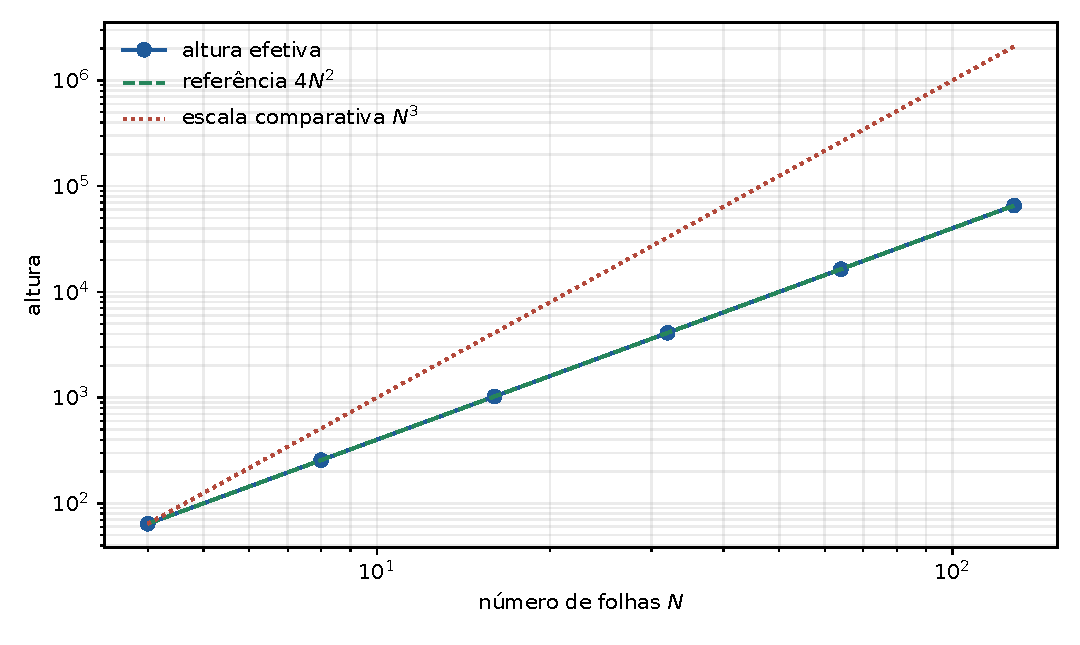
\includegraphics[width=.88\linewidth]{figuras/artigo_3/fig_altura_agendas.pdf}
 \caption{A altura efetiva da construção quadrática acompanha $N^2$; a
 curva $N^3$ corresponde ao fator de malha que o denominador comum absorve.}
 \label{artigo_3:fig:height-schedules}
\end{figure}

A \cref{artigo_3:fig:height-schedules} confirma, na construção quadrática auditada, a
separação entre a agenda provada $N^2$ e a escala comparativa $N^3$.

O programa \texttt{espacos\_aproximacao.py} usa
\texttt{fractions.Fraction} para reconstruir todos os valores nodais,
parâmetros, alturas e erros quadráticos. Ele verifica ainda, por enumeração
de $\mathcal Q_H$, a igualdade \eqref{artigo_3:eq:arithmetic-floor}; reproduz a
altura geométrica mínima $H=N$ das malhas uniformes em $[0,1]$; registra o
teste integral da série logarítmica; e emite o certificado simbólico da
\cref{artigo_3:prop:nonhomogeneous-functional}. Os testes são executados
independentemente da programação dinâmica das
seções de programação dinâmica do segundo artigo \citep{artigo_2-oliveiraII}.

\section{Reversibilidade regularizada e ponte quantitativa com redes ReLU}
\label{artigo_3:sec:regularized-reversibility}

Uma função linear por partes pode ser representada exatamente por uma rede ReLU
rasa por meio de uma expansão em hinges
\citep{artigo_2-devorehaninpetrova2021,artigo_1-daubechies2022}. Ela pode, portanto, ter poucas
folhas e, por isso, ter erro bruto nulo em todas as escalas posteriores sem
ganhar suavidade clássica. Essa barreira determina a forma dos teoremas
inversos desta seção.

Há três respostas, em níveis diferentes. Primeiro, o erro bruto admite uma
imersão inversa com perda, desde que se controle a inclinação efetivamente
realizada pelos aproximantes. Segundo, uma extensão marcada da biblioteca
remove a obstrução das regiões planas e dá uma equivalência exata com redes
ReLU rasas racionais de quebras diádicas; redes reais genéricas admitem uma
volta aproximada com recursos explícitos. Terceiro, usa-se um funcional de
realização, no sentido clássico de \citet{artigo_2-hristovivanov1990}, que soma ao erro
a autorregularidade do próprio aproximante. Nesse terceiro nível, a
desigualdade inversa é universal; a contribuição específica da biblioteca é o
lado direto de Jackson sob uma agenda explícita de altura racional.

A necessidade de orçar o crescimento dos coeficientes e a profundidade em
espaços de aproximação neural é enfatizada em
\citet{artigo_2-gribonval2022,artigo_2-grohs2023,artigo_1-guhring2021}. Em particular, o expoente crítico de Hölder
que surgirá no \cref{artigo_3:thm:raw-lossy-inverse} é a contraparte unidimensional e
uniforme do mecanismo de imersão de \citet{artigo_2-grohs2023}. As provas abaixo usam
apenas os módulos de suavidade e a altura da biblioteca.

\subsection{A obstrução que toda volta deve respeitar}

Escreva
\begin{equation}
 \psi(x)=\left|x-\frac12\right|,
 \qquad x\in[0,1].
 \label{artigo_3:eq:reverse-kink}
\end{equation}
Ela é uma montagem de duas folhas e altura $4$. Logo, para toda agenda que
eventualmente satisfaz $H(N)\ge4$,
\begin{equation}
 e_N^{\Library,H}(\psi)=0
 \quad\text{para todo $N$ suficientemente grande},
 \qquad
 \psi\in\mathscr A_q^\alpha(\Library,H)
 \quad(\alpha>0,\ 0<q\le\infty).
 \label{artigo_3:eq:kink-zero-raw-error}
\end{equation}
Por outro lado,
\begin{equation}
 \omega_2(\psi,h)_{\infty,[0,1]}=2h,
 \qquad 0<h\le\frac12,
 \label{artigo_3:eq:kink-exact-modulus-reverse}
\end{equation}
e, portanto,
\begin{equation}
 \psi\in B^s_{\infty,q}([0,1])
 \quad\Longleftrightarrow\quad
 s<1\ \text{ ou }\ (s=1\text{ e }q=\infty),
 \qquad 0<s<2.
 \label{artigo_3:eq:kink-besov-reverse}
\end{equation}
Com efeito, o salto de inclinação de $\psi$ é $2$, logo toda segunda diferença
de passo $h$ tem módulo no máximo $2h$; nos pontos
$1/2-h,1/2,1/2+h$ ela tem módulo exatamente $2h$. Substituir essa identidade
na caracterização diádica \eqref{artigo_3:eq:dyadic-besov-norm} prova
\eqref{artigo_3:eq:kink-besov-reverse}. Em particular, nenhum
teorema da forma
\begin{equation}
 e_N(f)=O(N^{-\alpha})\quad\Longrightarrow\quad
 f\in B^s_{\infty,q},
 \qquad s>1,
 \label{artigo_3:eq:forbidden-unregularized-converse}
\end{equation}
pode valer para o erro bruto do catálogo. Uma versão reversível deve conservar
informação sobre as quinas do aproximante, e não apenas sobre a distância de
$f$ a ele.

\subsection{A extensão marcada e a volta ReLU exata}

A inclinação nula foi
excluída da biblioteca original porque a imagem de um segmento constante não
recupera o suporte. Para estudar a volta, introduzimos uma extensão auxiliar
que guarda esse suporte como parte do código.

% MAPA artigo_3:5.1
\begin{definition}[biblioteca marcada completa]\label{map:artigo_3:5.1}
\label{artigo_3:def:marked-completion}
A biblioteca $\Library^\square$ é formada pelas quádruplas marcadas
\begin{equation}
 (k,m,y_0,s)\in\Nzero\times\mathbb Z\times\mathbb Q\times\mathbb Q,
 \label{artigo_3:eq:marked-atoms}
\end{equation}
com o mesmo segmento \eqref{artigo_3:eq:inherited-atom} e a mesma altura
\eqref{artigo_3:eq:inherited-height}. A marca $(k,m)$ é conservada na decodificação,
inclusive quando $s=0$. Denote por $\Aclass^\square(K)$ suas montagens
contínuas e por $\Aclass^\square_{N,H}(K)$ aquelas com no máximo $N$
folhas e altura atômica no máximo $H$.
\end{definition}

Tem-se $\Library\subset\Library^\square$. Para $s\ne0$, a marca é redundante
e a recuperação pela imagem coincide com a de $\Library$; para $s=0$, o
suporte é conservado explicitamente no par $(k,m)$.

Considere a forma ReLU reduzida
\begin{equation}
 R(x)=c+qx+\sum_{j=1}^{M}a_j\rho(x-\tau_j),
 \qquad 0<\tau_1<\cdots<\tau_M<1,
 \qquad a_j\ne0,
 \label{artigo_3:eq:reduced-relu-reverse}
\end{equation}
e suas inclinações locais
\begin{equation}
 \sigma_i=q+\sum_{j=1}^{i}a_j,
 \qquad 0\le i\le M.
 \label{artigo_3:eq:reverse-local-slopes}
\end{equation}
Para um conjunto finito $S\subset\mathbb D\cap(0,1)$, seja
$\mathcal T(S)$ a árvore diádica menos refinada cujas folhas não contêm
pontos de $S$ no interior. Ela é obtida subdividindo exatamente os ancestrais
necessários para transformar cada ponto de $S$ em fronteira.

% MAPA artigo_3:5.2
\begin{theorem}[reversibilidade rasa exata]\label{map:artigo_3:5.2}
\label{artigo_3:thm:exact-marked-reversal}
Uma função na forma reduzida \eqref{artigo_3:eq:reduced-relu-reverse} pertence a
$\Aclass^\square([0,1])$ se e somente se
\begin{equation}
 c,q,a_1,\ldots,a_M\in\mathbb Q,
 \qquad
 \tau_1,\ldots,\tau_M\in\mathbb D.
 \label{artigo_3:eq:marked-reversal-conditions}
\end{equation}
Nessas condições, $\mathcal T(\{\tau_1,\ldots,\tau_M\})$ é a única árvore
menos refinada que realiza $R$. Se $N_{\rm can}(R)$ é seu número de folhas e
$d_j$ é a profundidade diádica reduzida de $\tau_j$, então
\begin{equation}
 M+1\le N_{\rm can}(R)
 \le 1+\sum_{j=1}^{M}d_j.
 \label{artigo_3:eq:canonical-tree-leaf-bounds}
\end{equation}
A função pertence à biblioteca original $\Aclass([0,1])$ exatamente quando,
além de \eqref{artigo_3:eq:marked-reversal-conditions},
\begin{equation}
 \sigma_i\ne0\qquad(0\le i\le M).
 \label{artigo_3:eq:original-nonflat-condition}
\end{equation}
\end{theorem}

\begin{proof}
Suponha \eqref{artigo_3:eq:marked-reversal-conditions}. A árvore canônica transforma
todas as quebras em fronteiras. Em cada folha $J$, a função $R$ é afim, sua
inclinação é uma das $\sigma_i\in\mathbb Q$ e seu valor no centro é racional.
Esses dados determinam um átomo marcado; a continuidade de $R$ cola as peças.

Reciprocamente, toda montagem marcada é racional e afim no interior de cada
folha. Toda quebra real está em uma fronteira diádica, seu valor em $0$, a
inclinação inicial e os saltos de inclinação são racionais. Pela unicidade da
forma reduzida, obtém-se \eqref{artigo_3:eq:marked-reversal-conditions}.

Qualquer árvore que realize $R$ deve separar suas $M$ quebras reais, logo tem
ao menos $M+1$ folhas e refina $\mathcal T(S)$. Para inserir uma quebra de
profundidade $d_j$, bastam no máximo $d_j$ subdivisões novas. Como cada
subdivisão acrescenta uma folha, resulta a cota superior em
\eqref{artigo_3:eq:canonical-tree-leaf-bounds}. Finalmente, um átomo da biblioteca
original possui inclinação não nula; a condição é também suficiente folha a
folha.
\end{proof}

O teorema distingue duas contagens que coincidem apenas em partições já
alinhadas. $M+1$ conta regiões afins máximas; $N_{\rm can}$ conta células
diádicas. Por exemplo, uma única quebra em $1/4$ produz duas regiões, mas a
região $[1/4,1]$ precisa de duas folhas diádicas.

% MAPA artigo_3:5.3
\begin{definition}[altura canônica de rede]\label{map:artigo_3:5.3}
\label{artigo_3:def:canonical-network-height}
Para uma rede que satisfaz \eqref{artigo_3:eq:marked-reversal-conditions}, defina
\begin{equation}
 H_{\rm can}(R)=
 \max_{J_{k,m}\in\operatorname{leaf}(\mathcal T(S))}
 \max\{2,k+1,|m|+1,\height(R(x_{k,m})),\height(R'|_{J_{k,m}})\}.
 \label{artigo_3:eq:canonical-network-height}
\end{equation}
\end{definition}

Por construção, $H_{\rm can}(R)$ é exatamente a maior altura dos átomos na
montagem canônica. Essa é a medida que torna a ida e a volta isométricas no
recurso aritmético. A altura ingênua dos coeficientes
$(c,q,a_1,\ldots,a_M)$ não tem essa propriedade: somas de racionais podem
multiplicar denominadores.

% MAPA artigo_3:5.4
\begin{proposition}[forma ancorada e comprimento estrutural]\label{map:artigo_3:5.4}
\label{artigo_3:prop:anchored-relu-code}
Se $g\in\Aclass^\square_{N,H}([0,1])$, sua forma reduzida possui
$M\le N-1$ hinges e pode ser escrita, tomando o centro $x_*$ da folha mais à
esquerda, como
\begin{equation}
 g(x)=g(x_*)+\sigma_0(x-x_*)
      +\sum_{j=1}^{M}(\sigma_j-\sigma_{j-1})\rho(x-\tau_j).
 \label{artigo_3:eq:anchored-relu-form}
\end{equation}
Os valores $g(x_*)$ e $\sigma_i$ têm altura no máximo $H$, os saltos têm
altura no máximo $2H^2$, e os pontos diádicos são transmitidos por seus pares
estruturais. Consequentemente, existe uma codificação prefix-free da forma
ancorada com
\begin{equation}
 L_{\rm ReLU}^{\rm anc}(g)=O(N\log(2H)).
 \label{artigo_3:eq:anchored-network-bits}
\end{equation}

Na direção contrária, se os coeficientes de
\eqref{artigo_3:eq:reduced-relu-reverse} têm altura no máximo $W$ e as quebras têm
profundidade no máximo $D$ (e as quebras são diádicas em $(0,1)$), então
\begin{equation}
 H_{\rm can}(R)\le 2^{D+1}\,(M+2)\,W^{M+3},
 \qquad
 \log_2 H_{\rm can}(R)
 \le 5\bigl[(M+1)\log_2(2W)+D+\log_2(M+1)\bigr].
 \label{artigo_3:eq:reverse-height-bit-bound}
\end{equation}
\end{proposition}

\begin{proof}
Na ida, cada salto é a diferença de duas inclinações de altura no máximo
$H$, logo sua altura não excede $2H^2$. A altura atômica limita os inteiros
estruturais da célula, e todos os campos usam $O(\log(2H))$ bits. Somar os
$O(N)$ campos prova \eqref{artigo_3:eq:anchored-network-bits}, com constante explícita:
o código formalizado usa no máximo $40\,N\lfloor\log_2(2H)\rfloor$ bits. O ancoramento evita
expandir desnecessariamente $g(x_*)-\sigma_0x_*$ em um intercepto com
denominador diádico explícito.

Na volta, toda folha $J_{k,m}$ de $\mathcal T(S)$ tem $k\le D$ e
$|m|+1\le 2^k\le 2^D$. Cada inclinação local $\sigma_i$ é soma de no máximo $M+1$
racionais de altura $\le W$: um denominador comum é $\le W^{M+1}$ e
$|\sigma_i|\le(M+1)W$, logo $\operatorname{ht}\sigma_i\le (M+1)W^{M+2}$. O centro
$x_{k,m}=(2m+1)/2^{k+1}$ e as quebras têm denominador dividindo $2^{D+1}$, e
$0\le \max\{0,x_{k,m}-\tau_j\}\le1$. Assim, $R(x_{k,m})=c+qx_{k,m}+\sum_j
a_j\max\{0,x_{k,m}-\tau_j\}$ admite o denominador comum
$\operatorname{den}(c)\operatorname{den}(q)\,2^{D+1}\prod_j\operatorname{den}(a_j)\le
2^{D+1}W^{M+2}$ (a parte diádica é compartilhada por todas as parcelas) e módulo
$\le (M+2)W$; portanto $\operatorname{ht}R(x_{k,m})\le 2^{D+1}(M+2)W^{M+3}$. Os
demais termos de \eqref{artigo_3:eq:canonical-network-height} ($2$, $k+1\le D+1$,
$|m|+1\le 2^D$) são menores, o que dá $H_{\rm can}(R)\le 2^{D+1}(M+2)W^{M+3}$.
Tomando $\log_2$, e usando $W\ge1$, $\log_2(M+2)\le 1+\log_2(M+1)$ e
$(M+1)\log_2(2W)\ge1$, obtém-se
\[
 \log_2 H_{\rm can}\le D+1+\bigl(1+\log_2(M+1)\bigr)+(M+3)\log_2 W
 \le 5\bigl[(M+1)\log_2(2W)+D+\log_2(M+1)\bigr].
\]
\end{proof}

\begin{observacaoSN}\label{artigo_3:rem:reverse-height-correction}
O fator é $M+1$, e não $M$, no primeiro termo: há $M+1$ inclinações locais e
cada uma é soma de até $M+1$ racionais. A versão com $M\log(2W)$ é falsa já para
$M=0$: em $R(x)=x$ ($M=0$, $D=0$, $W=1$) tem-se $H_{\rm can}=2$, de modo que
$\log_2 H_{\rm can}=1$ e o lado direito é $0$; e em $R(x)=Wx$ tem-se
$H_{\rm can}\ge W$ (a altura da inclinação), de modo que nenhum termo constante
repara a cota. A volta corrigida está formalizada em
\texttt{Pendencias/AlturaInversa.lean}; a ida (forma ancorada e código prefix-free)
está formalizada em \texttt{Pendencias/FormaAncorada.lean} e
\texttt{Pendencias/CodigoAncorado.lean}.
\end{observacaoSN}

Assim, a reversibilidade exata preserva comprimento binário em ordem
polinomial, mas não preserva a altura ingênua coeficiente a coeficiente. A
altura correta do lado neural é \eqref{artigo_3:eq:canonical-network-height}, isto é,
o recurso aritmético depois da função ser colocada em sua partição diádica
canônica.

\subsection{Volta aproximada para redes rasas reais}

Quebras não diádicas e coeficientes irracionais impedem igualdade exata, mas
não uma conversão quantitativa. Cotas de erro e de recursos para aproximação
ReLU, inclusive sob restrições de codificação, são estudadas em
\citet{artigo_1-yarotsky2017,artigo_1-bolcskei2019}. A próxima estimativa dá uma forma explícita
da densidade compatível com a biblioteca.

% MAPA artigo_3:5.5
\begin{theorem}[reversão aproximada quantizada]\label{map:artigo_3:5.5}
\label{artigo_3:thm:quantized-approximate-reverse}
Seja $R$ como em \eqref{artigo_3:eq:reduced-relu-reverse}, agora com parâmetros reais,
e suponha
\begin{equation}
 |c|,|q|,|a_1|,\ldots,|a_M|\le W,
 \qquad W\ge1.
 \label{artigo_3:eq:real-network-weight-bound}
\end{equation}
Para todo $0<\varepsilon\le1$, existe uma montagem da biblioteca original
$g_\varepsilon\in\Aclass([0,1])$ tal que
\begin{align}
 \|R-g_\varepsilon\|_\infty&\le\varepsilon,
 \label{artigo_3:eq:approximate-reverse-error}\\
 |\Lambda(g_\varepsilon)|&\le1+MD_\varepsilon,
 \qquad
 D_\varepsilon=
 \left\lceil\log_2\frac{C(M+1)(W+1)}{\varepsilon}\right\rceil,
 \label{artigo_3:eq:approximate-reverse-leaves}\\
 \height_{\max}(g_\varepsilon)
 &\le
 C(M+1)^3(W+1)^3\varepsilon^{-2},
 \label{artigo_3:eq:approximate-reverse-height}
\end{align}
onde $C$ é universal. A conclusão permanece válida quando $R$ possui regiões
planas.
\end{theorem}

\begin{proof}
Ponha
\[
 \delta=\frac{\varepsilon}{16(M+1)(W+1)}.
\]
Escolha um denominador comum $Q\asymp\delta^{-1}$ e aproxime
$c,q,a_1,\ldots,a_M$ por múltiplos de $1/Q$ com erro no máximo $\delta$.
Aproxime cada $\tau_j$ por um diádico de profundidade
$D\le D_\varepsilon$. A função $z\mapsto\rho(x-z)$ é $1$-Lipschitz e
$0\le\rho(x-z)\le1$ em $[0,1]$, de modo que a soma dos erros de coeficientes
e deslocamentos é no máximo
\[
 (M+2)\delta+M(W+\delta)\delta.
\]
Nós que colidem são combinados; nós que chegam a $0$ são absorvidos no termo
linear e os que chegam a $1$ desaparecem no domínio.

Resta impedir inclinações locais nulas. Depois da quantização há no máximo
$M+1$ valores proibidos para uma perturbação global da inclinação. Entre
$M+2$ múltiplos positivos consecutivos de $1/Q$, escolha um que não seja
proibido e acrescente o termo correspondente $\eta x$. A escolha de $Q$ e a
folga em $\delta$ mantêm o erro total abaixo de $\varepsilon$.

A árvore canônica exige no máximo $1+MD$ folhas pelo
\cref{artigo_3:thm:exact-marked-reversal}. Inclinações locais têm denominador comum
$Q$ e numeradores $O((M+1)(W+1)Q)$. Valores nos centros têm denominador que
divide $Q2^{D+1}$ e numeradores
$O((M+1)(W+1)Q2^D)$. Como
$Q,2^D=O((M+1)(W+1)\varepsilon^{-1})$, segue
\eqref{artigo_3:eq:approximate-reverse-height}. A perturbação final permite usar a
biblioteca original, não apenas sua extensão marcada.
\end{proof}

% MAPA artigo_3:5.6
\begin{corollary}[redes profundas medidas pela função realizada]\label{map:artigo_3:5.6}
\label{artigo_3:cor:deep-functional-reverse}
Se uma rede ReLU univariada arbitrária realiza uma função $F$ com $R(F)$
regiões afins máximas, norma uniforme no máximo $B$ e constante de Lipschitz
no máximo $L_F$, então o \cref{artigo_3:thm:quantized-approximate-reverse} vale com
\begin{equation}
 M=R(F)-1,
 \qquad
 W\le2\max\{1,B,L_F\}.
 \label{artigo_3:eq:deep-realized-resources}
\end{equation}
\end{corollary}

\begin{proof}
Toda função ReLU univariada é linear por partes e admite a forma hinge rasa
canônica, independentemente da arquitetura que a produziu. A inclinação
inicial tem módulo no máximo $L_F$, cada salto tem módulo no máximo $2L_F$ e
$|F(0)|\le B$. Aplique o teorema anterior.
\end{proof}

A relação entre profundidade e número de regiões pode ser exponencial, como nas
construções de separação por profundidade de \citet{artigo_2-telgarsky2016}. Para o bloco
tenda
\[
 T(x)=2\rho(x)-4\rho(x-\tfrac12),\qquad x\in[0,1],
\]
a iterada $T_L=T^{\circ L}$ possui exatamente $2^L$ regiões afins máximas,
com inclinações $\pm2^L$: cada composição bissecta todas as regiões do nível
anterior. Assim, toda montagem que realize $T_L$ exatamente requer ao menos
$2^L$ folhas e altura atômica ao menos $2^L$. A dependência do corolário nos
recursos realizados conserva, portanto, essa separação exponencial.

A \cref{artigo_3:tab:deep-tent-network} explicita os primeiros oito níveis dessa lei,
e a \cref{artigo_3:fig:network-restrictions} contrasta número de blocos, regiões
realizadas e recursos mínimos da biblioteca.

\begin{table}[t]
 \centering
 \small
 \begin{tabular}{rrrr}
\toprule
profundidade $L$ & blocos & regiões/folhas mín. & altura mín.\\
\midrule
1 & 1 & 2 & 2\\
2 & 2 & 4 & 4\\
3 & 3 & 8 & 8\\
4 & 4 & 16 & 16\\
5 & 5 & 32 & 32\\
6 & 6 & 64 & 64\\
7 & 7 & 128 & 128\\
8 & 8 & 256 & 256\\
\bottomrule
\end{tabular}

 \caption{Separação exata para a tenda iterada: $L$ blocos produzem $2^L$
 regiões, e qualquer montagem exata requer ao menos $2^L$ folhas e altura
 atômica ao menos $2^L$.}
 \label{artigo_3:tab:deep-tent-network}
\end{table}

\begin{figure}[t]
 \centering
 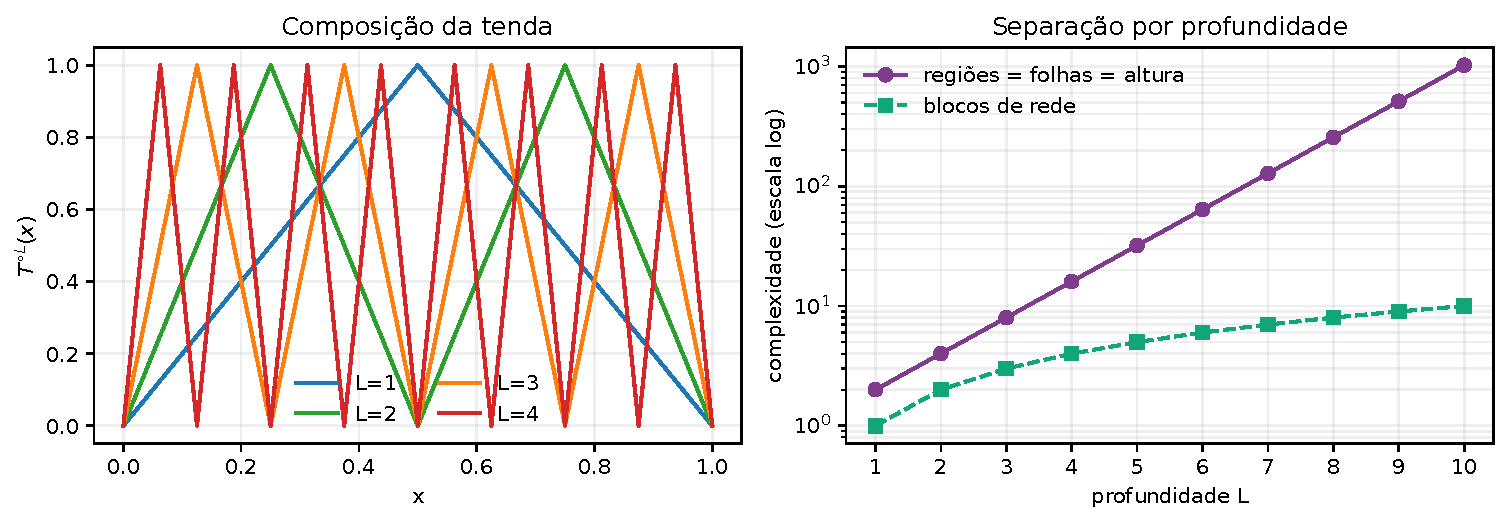
\includegraphics[width=.88\linewidth]{figuras/artigo_3/fig_restricoes_rede.pdf}
 \caption{Crescimento dos recursos realizados pela tenda iterada. Os pontos
 provêm de identidades exatas; as linhas apenas guiam a leitura.}
 \label{artigo_3:fig:network-restrictions}
\end{figure}

\begin{table}[t]
 \centering
 \small
 \begin{tabular}{rrrrrr}
\toprule
$M$ & $\varepsilon$ & $D$ & folhas & cota de folhas & erro/$\varepsilon$\\
\midrule
1 & $1/32$ & 12 & 13 & 13 & 0.0099\\
1 & $1/64$ & 13 & 14 & 14 & 0.0037\\
1 & $1/128$ & 14 & 15 & 15 & 0.0131\\
1 & $1/32$ & 11 & 12 & 12 & 0.0245\\
1 & $1/64$ & 12 & 13 & 13 & 0.0099\\
1 & $1/128$ & 13 & 14 & 14 & 0.0120\\
\bottomrule
\end{tabular}

 \caption{Auditoria racional da reversão aproximada. As redes de entrada
 possuem quebras não diádicas. O erro é calculado exatamente no conjunto
 unido de quebras, onde o máximo de uma diferença linear por partes é
 atingido.}
 \label{artigo_3:tab:approximate-reverse-audit}
\end{table}

Os casos quantizados da \cref{artigo_3:tab:approximate-reverse-audit} verificam, com
frações exatas, a cota de erro e a permanência na biblioteca original.

\subsection{A melhor recíproca para o erro bruto}

Todo $g\in\Sigma_N^{\Library,H}$ é $H(N)$-Lipschitz, pois em cada folha sua
inclinação $s$ satisfaz $|s|\le\height(s)\le H(N)$. Consequentemente,
$\omega_2(g,t)_\infty\le2H(N)t$. Essa desigualdade de tipo Bernstein contém
uma recíproca verdadeira, desde que se aceite a perda imposta pelo crescimento
das inclinações. A formulação seguinte não depende da aritmética.

% MAPA artigo_3:5.7
\begin{theorem}[imersão inversa sob crescimento de Lipschitz]\label{map:artigo_3:5.7}
\label{artigo_3:thm:raw-lossy-inverse}
Sejam $\mathcal G_N\subset C([0,1])$ famílias de aproximantes tais que
\begin{equation}
 \operatorname{Lip}(g)\le C_LN^\gamma
 \qquad(g\in\mathcal G_N),
 \qquad \gamma\ge0,
 \label{artigo_3:eq:lipschitz-growth-family}
\end{equation}
e defina
$e_N^{\mathcal G}(f)=\inf_{g\in\mathcal G_N}\|f-g\|_\infty$. Se
\begin{equation}
 A_\alpha(f):=\sup_{N\ge1}N^\alpha e_N^{\mathcal G}(f)<\infty,
 \qquad \alpha>0,
 \label{artigo_3:eq:raw-rate-assumption}
\end{equation}
então, com
\begin{equation}
 \theta_* = \frac{\alpha}{\alpha+\gamma},
 \label{artigo_3:eq:critical-reverse-exponent}
\end{equation}
vale
\begin{equation}
 \omega_2(f,t)_\infty
 \le C_{\alpha,\gamma}(A_\alpha(f)+C_L)t^{\theta_*},
 \qquad 0<t\le\frac12.
 \label{artigo_3:eq:raw-inverse-modulus}
\end{equation}
Consequentemente,
\begin{equation}
 f\in B^{\theta_*}_{\infty,\infty}([0,1])
 \quad\text{e}\quad
 f\in B^\theta_{\infty,r}([0,1])
 \quad(0<\theta<\theta_*,\ 0<r\le\infty).
 \label{artigo_3:eq:raw-inverse-besov}
\end{equation}
\end{theorem}

\begin{proof}
Para qualquer $g\in\mathcal G_N$, a desigualdade triangular para segundas
diferenças e a propriedade Lipschitz dão
\begin{equation}
 \omega_2(f,t)_\infty
 \le4\|f-g\|_\infty+2C_LN^\gamma t.
 \label{artigo_3:eq:inverse-balance}
\end{equation}
Escolha $N$ comparável a $t^{-1/(\alpha+\gamma)}$ e use um aproximante
arbitrariamente próximo do ínfimo. Os dois termos do lado direito passam a
ser $O(t^{\alpha/(\alpha+\gamma)})$, o que prova
\eqref{artigo_3:eq:raw-inverse-modulus}. A caracterização diádica de Besov fornece o
endpoint por supremo. Para $\theta<\theta_*$, a sequência normalizada ganha o
fator geométrico $2^{-j(\theta_*-\theta)}$ e pertence a todo $\ell^r$.
\end{proof}

% MAPA artigo_3:5.8
\begin{corollary}[aplicação às agendas diretas]\label{map:artigo_3:5.8}
\label{artigo_3:cor:raw-library-inverse}
Se $H(N)\le C N^\gamma$, então
\begin{equation}
 \mathscr A_q^\alpha(\Library,H)
 \subset B^{\alpha/(\alpha+\gamma)}_{\infty,\infty}([0,1]),
 \qquad 0<q\le\infty.
 \label{artigo_3:eq:raw-library-inverse}
\end{equation}
Para as agendas $H_{s,0}$ da \cref{artigo_3:sec:direct-height}, isso dá
\begin{equation}
 \mathscr A_q^s(\Library,H_{s,0})
 \subset B^{\vartheta_s}_{\infty,\infty},
 \qquad
 \vartheta_s=
 \begin{cases}
 s/(s+1),&0<s<1,\\
 1/2,&1\le s<2.
 \end{cases}
 \label{artigo_3:eq:corrected-schedule-raw-inverse}
\end{equation}
Se a agenda possui ainda um fator logarítmico, a mesma conclusão vale para
toda ordem estritamente menor que $\vartheta_s$.
\end{corollary}

\begin{proof}
Todo elemento de $\Sigma_N^{\Library,H}$ é $H(N)$-Lipschitz. O funcional com
$q<\infty$ controla o de supremo pela redução diádica do
\cref{artigo_3:thm:dyadic-rate-equivalence}. Um fator logarítmico é dominado por
$N^\eta$ para qualquer $\eta>0$; aplique o teorema com
$\gamma+\eta$ e faça $\eta\downarrow0$.
\end{proof}

O \cref{artigo_3:thm:critical-tent-comb} realiza o expoente \eqref{artigo_3:eq:critical-reverse-exponent} na biblioteca original, com inclinações locais não nulas, na faixa $0<\alpha\le\gamma$.

% MAPA artigo_3:5.9
\begin{theorem}[agudeza por um pente de tendas]\label{map:artigo_3:5.9}
\label{artigo_3:thm:critical-tent-comb}
Fixe $0<\alpha\le\gamma$ e ponha
$\theta_*=\alpha/(\alpha+\gamma)$. Existe
$f\in C([0,1])$ e uma constante $C$ tais que, para a biblioteca original sob
$H(N)=\lceil CN^\gamma\rceil$,
\begin{equation}
 e_N^{\Library,H}(f)\le CN^{-\alpha},
 \label{artigo_3:eq:comb-approximation-rate}
\end{equation}
mas
\begin{equation}
 f\notin B^\theta_{\infty,\infty}\quad(\theta>\theta_*),
 \qquad
 f\notin B^{\theta_*}_{\infty,r}\quad(0<r<\infty).
 \label{artigo_3:eq:comb-sharpness}
\end{equation}
\end{theorem}

\begin{proof}
Escolha um inteiro $J_0$ tão grande que
$J_0(\alpha+\gamma)>3$. Para $j\ge1$, ponha
\[
 a_j=\lceil J_0\alpha j\rceil,
 \qquad b_j=\lfloor J_0\gamma j\rfloor,
 \qquad r_j=a_j+b_j-1.
\]
No intervalo diádico $J_{r_j,1}$, coloque uma tenda $\phi_j$ de altura
$2^{-a_j}$, nula nas extremidades e linear em cada metade. As escolhas
garantem que os suportes são disjuntos e acumulam apenas em $0$. Defina
$f=\sum_{j\ge1}\phi_j$.

A inclinação da $j$-ésima tenda tem módulo $2^{b_j}$ e os valores centrais de
suas duas metades têm altura $2^{a_j+1}$. Seja $T_j$ a árvore diádica em pente
que isola as duas metades das primeiras $j$ tendas. Ela possui
$O(r_j+j)$ folhas; fora dessas tendas, a soma parcial
$f_j=\sum_{i\le j}\phi_i$ é nula em cada folha restante.

Para eliminar todas as inclinações nulas sem alterar o alvo $f$, subdivida uma
vez cada folha plana $J$ de $T_j$ e, sobre $J$, acrescente uma tenda
$\psi_{J,j}$ nula nos extremos e de altura
\[
 \delta_j=2^{-a_{j+1}-2}
\]
no ponto médio. Os suportes dessas pequenas tendas são disjuntos. A função
\[
 g_j=f_j+\sum_{J\ {\rm plano\ em}\ T_j}\psi_{J,j}
\]
é contínua e tem inclinação não nula em toda folha da árvore refinada. Logo
$g_j$ é uma montagem da biblioteca original, não da extensão marcada.

Resta conferir os dois orçamentos. A árvore refinada tem ainda
$O(r_j+j)$ folhas. Em uma folha plana de profundidade $d\le r_j+1$, a nova
inclinação tem módulo $2^{d+1}\delta_j$; sua altura é limitada por
\[
 \max\{2^{a_{j+1}+1},\,2^{r_j-a_{j+1}}\}
 \le C2^{J_0\gamma j}.
\]
Os valores centrais novos têm altura no máximo $2^{a_{j+1}+3}$, e os
parâmetros das tendas originais são limitados por
$C\max\{2^{a_j},2^{b_j}\}$. As células profundas do pente têm índices
$m\in\{0,1,2,3\}$; portanto escala e translação obedecem à mesma cota.
Como $\alpha\le\gamma$, todos esses termos são no máximo
$CN_j^\gamma$ para $N_j=2^{J_0j}$, depois de aumentar $C$. Também
$O(r_j+j)\le N_j$ para $j$ grande; as finitíssimas escalas iniciais são
absorvidas em $C$ e por uma reindexação finita.

Por disjunção dos suportes,
\[
 \|f-g_j\|_\infty
 \le \Bigl\|\sum_{i>j}\phi_i\Bigr\|_\infty+\delta_j
 \le 2^{-a_{j+1}}+\delta_j
 \le C N_j^{-\alpha}.
\]
Para $N_j\le N<N_{j+1}$, use $g_j$; a razão
$N_{j+1}/N_j=2^{J_0}$ é fixa. A monotonicidade da agenda e o ajuste dessa
constante provam \eqref{artigo_3:eq:comb-approximation-rate} para todo $N$.

Se $h_j=2^{-(r_j+1)}$ é a meia-largura da tenda, os valores
$0,2^{-a_j},0$ dão
\[
 \omega_2(f,h_j)_\infty\ge2^{1-a_j}\asymp h_j^{\theta_*}.
\]
Isso exclui toda ordem maior no supremo e torna constante uma subsequência do
coeficiente crítico, que não pertence a nenhum $\ell^r$ finito.
\end{proof}

A exigência $\alpha\le\gamma$ cobre em particular as agendas críticas da
\cref{artigo_3:sec:direct-height}. Ela também expõe por que a informação correta é a inclinação
realizada, não a altura do endereço isoladamente.

\subsection{Funcional de realização: lado direto com altura controlada}

A agudeza do teorema anterior fixa a regularidade determinada pelo erro bruto
e por uma cota de Lipschitz. Para comparar com a suavidade clássica, considere
o funcional de realização associado ao módulo de segunda ordem. Funcionais
desse tipo foram introduzidos para substituir $K$-funcionais degenerados em
aproximação restrita \citep{artigo_2-hristovivanov1990}. Para $N\ge2$, defina
\begin{equation}
 \mathcal R_N^{\Library,H}(f)
 :=\inf_{g\in\Sigma_N^{\Library,H}([0,1])}
 \left\{\|f-g\|_\infty+
 \omega_2(g,N^{-1})_\infty\right\}.
 \label{artigo_3:eq:self-roughness-certificate}
\end{equation}
O primeiro termo mede fidelidade; o segundo impede que uma função com quinas
receba suavidade apenas porque já pertence ao catálogo.

% MAPA artigo_3:5.10
\begin{lemma}[desigualdade inversa universal]\label{map:artigo_3:5.10}
\label{artigo_3:lem:universal-regularized-inverse}
Para toda agenda, toda $f\in C([0,1])$ e todo $N\ge2$,
\begin{equation}
 \frac14\omega_2(f,N^{-1})_\infty
 \le \mathcal R_N^{\Library,H}(f).
 \label{artigo_3:eq:universal-regularized-lower}
\end{equation}
\end{lemma}

\begin{proof}
Para qualquer $g$ admissível,
\[
 \omega_2(f,N^{-1})_\infty
 \le4\|f-g\|_\infty+\omega_2(g,N^{-1})_\infty
 \le4\bigl(\|f-g\|_\infty+\omega_2(g,N^{-1})_\infty\bigr).
\]
Tome o ínfimo.
\end{proof}

% MAPA artigo_3:5.11
\begin{remark}[o que o funcional mede]\label{map:artigo_3:5.11}
\label{artigo_3:rem:realization-functional-scope}
A cota inversa decorre da desigualdade triangular para segundas diferenças e vale para qualquer família de candidatos. O lado direto usa a biblioteca para construir aproximantes sob a agenda aritmética da \cref{artigo_3:sec:direct-height}.
\end{remark}

% MAPA artigo_3:5.12
\begin{theorem}[Jackson racional para o funcional de realização]\label{map:artigo_3:5.12}
\label{artigo_3:thm:regularized-jackson-bernstein}
Se $0<s<2$ e $f\in B^s_{\infty,\infty}([0,1])$, então, para toda potência de
dois $N$ suficientemente grande e toda altura que satisfaz as hipóteses do
\cref{artigo_3:lem:rational-jackson-height},
\begin{equation}
 \frac14\omega_2(f,N^{-1})_\infty
 \le \mathcal R_N^{\Library,H}(f)
 \le C_0\omega_2(f,N^{-1})_\infty+\frac{C_f}{H(N)},
 \label{artigo_3:eq:two-sided-regularized-equivalence}
\end{equation}
onde $C_0$ é universal e $C_f$ depende apenas de $\|f\|_\infty$ e das
constantes fixadas na racionalização.
Se $\|f\|_{B^s_{\infty,\infty}}^*\le B$, $B\ge1$, e
$H(N)\ge\widehat H_{s,0}^{[B]}(N)$, a mesma estimativa vale para toda potência
diádica $N\ge2$, com $C_f/H(N)$ substituído por $C(B+1)/H(N)$ e constantes
independentes de $f$.
\end{theorem}

\begin{proof}
A cota inferior é o lema anterior. Para a superior, tome o aproximante
racional $g_{N,H}$ do \cref{artigo_3:lem:rational-jackson-height}. Ele satisfaz
\[
 \|f-g_{N,H}\|_\infty
 \le2C_W\omega_2(f,N^{-1})_\infty+C_fH(N)^{-1}.
\]
Além disso, a desigualdade triangular aplicada na direção contrária dá
\[
 \omega_2(g_{N,H},N^{-1})_\infty
 \le\omega_2(f,N^{-1})_\infty+4\|f-g_{N,H}\|_\infty.
\]
Somar as duas estimativas e usar $g_{N,H}$ na definição de
$\mathcal R_N$ prova a cota superior. Na versão sobre a bola, aplique a parte
uniforme do mesmo lema; ela substitui o termo de quantização por
$8(B+1)/H(N)$ em todas as escalas diádicas, e o mesmo cálculo apenas altera a
constante universal.
\end{proof}

Defina o estrato reversível
\begin{equation}
 \mathscr R_q^s(\Library,H)
 :=\left\{f\in C([0,1]):
 \left\|\bigl(2^{rs}\mathcal R_{2^r}^{\Library,H}(f)\bigr)_{r\ge1}
 \right\|_{\ell^q}<\infty\right\}.
 \label{artigo_3:eq:reversible-stratum}
\end{equation}

% MAPA artigo_3:5.13
\begin{theorem}[caracterização pelo funcional de realização]\label{map:artigo_3:5.13}
\label{artigo_3:thm:complete-besov-reversibility}
Para $0<s<2$, valem as igualdades de conjuntos
\begin{align}
 B^s_{\infty,\infty}([0,1])
 &=\mathscr R_\infty^s(\Library,H_{s,0}),
 \label{artigo_3:eq:complete-reverse-endpoint}\\
 B^s_{\infty,q}([0,1])
 &=\mathscr R_q^s(\Library,H_{s,0}),
 &&0<q<\infty,\quad0<s<1,
 \label{artigo_3:eq:complete-reverse-subcritical}\\
 B^s_{\infty,q}([0,1])
 &=\mathscr R_q^s(\Library,H_{s,\kappa}),
 &&0<q<\infty,\quad1\le s<2,\quad\kappa>1/q.
 \label{artigo_3:eq:complete-reverse-critical}
\end{align}
Pode-se substituir a agenda logarítmica da última linha por qualquer agenda
com folga polinomial \eqref{artigo_3:eq:polynomial-slack-schedule}.
\end{theorem}

\begin{proof}
Se o funcional em \eqref{artigo_3:eq:reversible-stratum} é finito, a desigualdade
universal do \cref{artigo_3:lem:universal-regularized-inverse}, na forma
\eqref{artigo_3:eq:universal-regularized-lower}, e a caracterização diádica
\eqref{artigo_3:eq:dyadic-besov-norm} dão imediatamente
$f\in B^s_{\infty,q}$.

Na direção direta, aplique a cota superior. O termo do módulo pertence a
$\ell^q$ pela definição de Besov. Para $s<1$,
\[
 \frac{N^s}{H_{s,0}(N)}=O(N^{s-1}),
\]
que é geometricamente somável nas potências de dois. Para $q=\infty$ e
$s\ge1$, $N^s/H_{s,0}(N)$ é limitado. Para $q<\infty$ e $s\ge1$, a agenda
logarítmica produz $(\log(eN))^{-\kappa}$, cuja subsequência diádica pertence
a $\ell^q$ exatamente sob $\kappa q>1$. A folga polinomial produz
$N^{-\eta}$. Um número finito de escalas iniciais não altera pertinência.
\end{proof}

O dado adicional que torna a taxa reversível é a segunda diferença do próprio
aproximante na escala pareada. A altura permanece aritmética e usa as agendas
da \cref{artigo_3:sec:direct-height}; a uniformidade quantitativa sobre bolas é dada
pelos \cref{artigo_3:thm:direct-besov-height,artigo_3:cor:uniform-besov-ball-embedding}. A caracterização refere-se ao funcional de realização.

Para a quina \eqref{artigo_3:eq:reverse-kink}, tomar $g=\psi$ zera o primeiro termo,
mas deixa
\begin{equation}
 \mathcal R_N^{\Library,H}(\psi)
 \le\omega_2(\psi,N^{-1})_\infty=\frac2N.
 \label{artigo_3:eq:kink-regularized-rate}
\end{equation}
A cota universal mostra a mesma ordem. Logo a taxa reversível é exatamente
um, em acordo com \eqref{artigo_3:eq:kink-besov-reverse}, e não infinita.

\begin{table}[t]
 \centering
 \small
 \begin{tabular}{rrrrr}
\toprule
$N$ & $e_N(\psi)$ & $\omega_2(\psi,N^{-1})$ & $N\omega_2$ & $N^{3/2}\omega_2$\\
\midrule
4 & 0 & $1/2$ & 2.000 & 4.000\\
8 & 0 & $1/4$ & 2.000 & 5.657\\
16 & 0 & $1/8$ & 2.000 & 8.000\\
32 & 0 & $1/16$ & 2.000 & 11.314\\
64 & 0 & $1/32$ & 2.000 & 16.000\\
128 & 0 & $1/64$ & 2.000 & 22.627\\
\bottomrule
\end{tabular}

 \caption{A quina sob o erro bruto e a parcela de autorregularidade obtida
 com o candidato $g=\psi$. Embora $e_N(\psi)=0$, essa parcela é $2/N$; a
 cota universal \eqref{artigo_3:eq:universal-regularized-lower} garante que o ínfimo
 completo tem a mesma ordem $N^{-1}$.}
 \label{artigo_3:tab:kink-regularized-certificate}
\end{table}

A \cref{artigo_3:tab:kink-regularized-certificate} torna explícita a diferença entre
erro bruto nulo e autorregularidade de ordem $N^{-1}$.

\subsection{Estabilidade da caracterização ao ampliar a arquitetura}

O certificado é definido no espaço de funções, independentemente de uma
parametrização neural, o que permite comparar famílias arquiteturais inteiras.

% MAPA artigo_3:5.14
\begin{theorem}[reversibilidade estável por inclusão de redes]\label{map:artigo_3:5.14}
\label{artigo_3:thm:architecture-stable-reversibility}
Seja $(\mathcal N_N)$ qualquer família de funções realizadas por redes ReLU
aninhada no orçamento, isto é,
\begin{equation}
 0\in\mathcal N_N,
 \qquad \mathcal N_N\subseteq\mathcal N_{N+1}
 \qquad(N\ge1),
 \label{artigo_3:eq:network-family-nesting}
\end{equation}
e suponha que, para alguma constante $c\ge1$,
\begin{equation}
 \Sigma_N^{\Library,H}([0,1])\subseteq\mathcal N_{\lceil cN\rceil}
 \qquad(N\ge1).
 \label{artigo_3:eq:network-family-contains-library}
\end{equation}
Defina
\begin{equation}
 \mathcal R_N^{\mathcal N}(f)
 =\inf_{R\in\mathcal N_N}
 \left\{\|f-R\|_\infty+\omega_2(R,N^{-1})_\infty\right\}.
 \label{artigo_3:eq:network-regularized-certificate}
\end{equation}
Sob cada uma das agendas do
\cref{artigo_3:thm:complete-besov-reversibility}, substituir
$\mathcal R_N^{\Library,H}$ por $\mathcal R_N^{\mathcal N}$ preserva as
igualdades \eqref{artigo_3:eq:complete-reverse-endpoint}--
\eqref{artigo_3:eq:complete-reverse-critical}.
\end{theorem}

\begin{proof}
A desigualdade inversa
\[
 \omega_2(f,N^{-1})_\infty\le4\mathcal R_N^{\mathcal N}(f)
\]
vale para toda função contínua $R$, independentemente da arquitetura. Essa é
a inclusão do estrato neural no Besov. Na direção direta, realize na família
neural o aproximante racional da
\cref{artigo_3:thm:regularized-jackson-bernstein}. Ponha
$d=2^{\lceil\log_2c\rceil}$. Para todo orçamento diádico $M=2^r\ge d$, o
número $n=M/d$ é também uma potência de dois e
$\lceil cn\rceil\le M$. Por \eqref{artigo_3:eq:network-family-contains-library} e pelo
aninhamento \eqref{artigo_3:eq:network-family-nesting},
\[
 \Sigma_n^{\Library,H}([0,1])
 \subseteq\mathcal N_{\lceil cn\rceil}
 \subseteq\mathcal N_M.
\]
Se $g_{n,H}$ é o aproximante usado naquele teorema, a monotonicidade do módulo
na escala fornece
\begin{align*}
 \mathcal R_M^{\mathcal N}(f)
 &\le \|f-g_{n,H}\|_\infty+\omega_2(g_{n,H},M^{-1})_\infty\\
 &\le \|f-g_{n,H}\|_\infty+\omega_2(g_{n,H},n^{-1})_\infty\\
 &\le C_0\omega_2(f,n^{-1})_\infty+\frac{C_f}{H(n)}.
\end{align*}
Como $M=dn$, multiplicar por $M^s$ introduz apenas o fator fixo $d^s$, e a
passagem de $M$ a $n$ desloca por $\log_2d$ índices as sequências diádicas.
As mesmas estimativas de $\ell^q$ da
\cref{artigo_3:thm:complete-besov-reversibility} concluem a direção direta. Um número
finito de escalas $M<d$ não afeta o estrato.
\end{proof}

Pelo \cref{artigo_3:thm:architecture-stable-reversibility}, ampliar a família de redes preserva a caracterização: a cota inferior depende do módulo do alvo. Redes profundas podem reduzir o erro, mas o certificado permanece maior ou igual a um quarto desse módulo.

\begin{figure}[t]
 \centering
 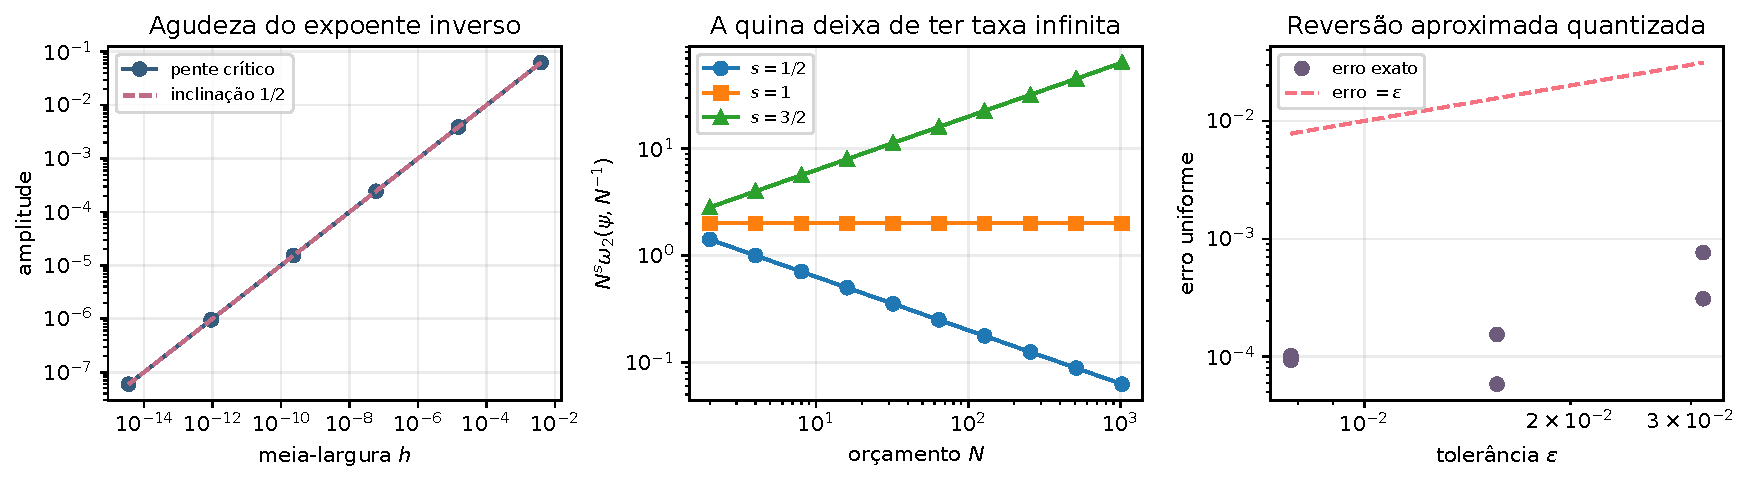
\includegraphics[width=.98\linewidth]{figuras/artigo_3/fig_reversibilidade_regularizada.pdf}
 \caption{Três diagnósticos da reversibilidade. À esquerda, o pente de tendas
 realiza o expoente crítico $\alpha/(\alpha+\gamma)$. Ao centro, o certificado
 atribui à quina exatamente a ordem um. À direita, a quantização de redes com
 quebras não diádicas permanece abaixo da tolerância prescrita.}
 \label{artigo_3:fig:regularized-reversibility}
\end{figure}

Os três mecanismos aparecem lado a lado na
\cref{artigo_3:fig:regularized-reversibility}; o painel do pente usa a
construção na biblioteca original do \cref{artigo_3:thm:critical-tent-comb}.

\subsection{Validação executável}

O programa \texttt{reversibilidade\_regularizada.py} executa uma auditoria
independente em aritmética \texttt{Fraction}. Ele:
\begin{enumerate}[label=(\roman*),leftmargin=2.2em]
 \item executa $2952$ idas e voltas exatas entre formas hinge e árvores
 canônicas, das quais $1160$ contêm ao menos uma região plana;
 \item verifica em todos os casos as duas cotas de folhas de
 \eqref{artigo_3:eq:canonical-tree-leaf-bounds};
 \item quantiza $84$ redes com quebras não diádicas e confere exatamente erro,
 número de folhas, inclinações não nulas e altura;
 \item testa $1260$ instâncias da desigualdade universal que sustenta
 \eqref{artigo_3:eq:universal-regularized-lower};
 \item reproduz a quina em dez escalas, a tenda profunda até $1024$ regiões e
 seis níveis do pente crítico, verificando em cada nível a perturbação, o erro,
 a altura, o número de folhas e a ausência de inclinações nulas na biblioteca
 original.
\end{enumerate}

A reversibilidade assume três formas. A biblioteca $\Library$ corresponde
exatamente à imagem rasa caracterizada por dados racionais, nós diádicos e
inclinações não nulas. A extensão marcada inclui regiões planas e produz uma
bijeção funcional rasa. Redes reais genéricas admitem aproximações inversas
com recursos explícitos. No nível de classes funcionais, o erro bruto possui a recíproca com perda do
\cref{artigo_3:thm:raw-lossy-inverse}, enquanto o certificado
\eqref{artigo_3:eq:self-roughness-certificate} fornece a caracterização direta e
inversa completa do \cref{artigo_3:thm:complete-besov-reversibility}. Essas três formas
separam representação exata, quantização e regularidade funcional.
\section{Conclusão}
As agendas de altura acompanham simultaneamente a geometria da malha e a quantização racional. A construção direta usa o expoente $\max\{1,s\}$ e, na faixa crítica com $q<\infty$, um fator logarítmico suficiente para a somabilidade. O piso aritmético uniforme exige crescimento de ordem $N^s$ quando a classe contém um intervalo de funções constantes.

O erro bruto e o crescimento das inclinações fornecem a regularidade inversa $\alpha/(\alpha+\gamma)$, aguda na biblioteca original para $0<\alpha\le\gamma$. A representação exata por redes rasas depende da racionalidade dos parâmetros e da posição diádica das quebras; redes com parâmetros reais admitem uma conversão aproximada com recursos explícitos.

O funcional de realização conserva a informação de segunda ordem que o melhor erro isolado perde. Sua cota inversa universal e o lado direto racional caracterizam os estratos de Besov sob as agendas declaradas. A mesma caracterização permanece válida para famílias de redes que contêm os aproximantes da biblioteca com sobrecusto linear de orçamento.


